% !TeX root = RJwrapper.tex
\title{Crowdsourced Data Preprocessing with R and Amazon Mechanical Turk}
\author{by Thomas J. Leeper}

\maketitle

\abstract{This article introduces the use of the Amazon Mechanical Turk (MTurk) crowdsourcing platform as a resource for R users to preprocess ``messy'' data into a form easily analyzed within R. The article first describes MTurk and the \CRANpkg{MTurkR} package, then outlines how to use \pkg{MTurkR} to gather and manage crowdsourced data with MTurk using some of the package's core functionality. Potential applications of \pkg{MTurkR} include construction of manually coded training sets, human transcription and translation, manual data scraping from scanned documents, content analysis, image classification, and the completion of online survey questionnaires, among others. As an example of massive data preprocessing, the article describes an image rating task involving 225 crowdsourced workers and more than 5500 images using just three \pkg{MTurkR} function calls.}

\section{Introduction}

People use R because it is extensible, robust, and free. It can do many things, but doing those many things generally requires data structures that can be handled computationally. Yet R users are often faced with messy data that are not R-ready: handwritten survey responses, digitized texts that cannot be read by optical character recognition, images, etc. Or an analyst may face machine readable data but require human interpretation to categorize, translate, or code those data, such as someone wishing to build an automated classifier needs a human-categorized training set to test their implementation.

In such cases, making the leap from these raw data to R data structures can entail considerable human labor. Such needs for human labor in data preprocessing has provoked interest in online crowdsourcing platforms \citep{Schmidt2010, ChenMenezesBradley2011} to bring human intelligence to tasks that cannot be easily accomplished through computation alone. This paper describes the use of \CRANpkg{MTurkR} \citep{Leeper2012c} to leverage the Amazon Mechanical Turk (MTurk) crowdsourcing platform to bring human intelligence into R. The article begins by laying out the need for occasional human intelligence in data preprocessing, then describes MTurk and its vocabulary, and introduces \pkg{MTurkR}. The remainder of the article describes the use of \pkg{MTurkR} for crowdsourced data preprocessing.

\section{The Need for Human Intelligence}
Some data cannot be computationally processed. Other data can be handled only with difficulty. In such cases, manual data processing often comes at the cost of time, money, and effort. Archetypal needs for human intelligence include the collection of data which cannot be automated (e.g., online data that lacks the well-defined structure to be scraped and parsed as XML or JSON), the preprocessing of ``messy'' data in formats that cannot be directly analyzed (e.g., handwritten documents scanned as PDFs), tasks that are laborious to translate from an R-readable but non-computable data structure into a format that can be readily analyzed (e.g., long, text answers to free-response survey questions), or massive-scale machine readable data that require human interpretation (e.g., the data used in generating a training set for supervised learning algorithms).

Due to the manual nature of these tasks, processing such data can become challenging as the size of the dataset increases. Crowdsourcing these data preprocessing needs is therefore one way to obtain the scalable human intelligence needed to process even very large ``messy'' datasets. As opposed to an analyst engaged in manual preprocessing, crowdsourcing offers the possibility to leverage multiple sources of human intelligence, in parallel, thereby improving reliability and speed. Amazon Mechanical Turk (MTurk) stands out as one of the largest crowdsourcing platforms currently available and, given its powerful API, it is now accessible directly in R through \pkg{MTurkR}.

\section{MTurk: Introduction and Core Concepts}
Amazon Mechanical Turk is a crowdsourcing platform designed by Amazon.com as part of its suite of Amazon Web Service (AWS) tools to provide human intelligence for tasks that cannot be readily, affordably, or feasibly automated \citep{Amazon2012}. Because MTurk provides the web application for recruiting, paying, and managing human workers, the effort necessary to move a data cleaning task into the cloud is relatively effortless and can, in large part, be managed directly in R. While many early adopters of MTurk as a data generation tool have come from computer science \citep{MasonSuri2011, KitturChiSuh2008}, more recent attention has also emerged among social scientists who see MTurk's pool of workers as more than an affordable source of human labor \citep{BuhrmesterKwangGosling2011, BerinskyHuberLenz2010, PaolacciChandlerStern2010}. This article provides a sufficiently general overview of MTurk and \pkg{MTurkR} to enable its use for a variety of purposes, but focuses primarily on the uses of MTurk for data preprocessing.\footnote{Users specifically interested in social science survey and experimental applications should consult \citet{Leeper2013a} and the \pkg{MTurkR} documentation.}

\subsection{Key Terms and Concepts}
MTurk connects \dfn{requesters}, who are willing to pay \dfn{workers} to perform a given task or set of tasks at a specified price per task. These ``Human Intelligence Tasks'' (HITs), are the core element of the MTurk platform. A HIT is a task that a requester would like one or more workers to perform. Every HIT is automatically assigned a unique HITId to identify this HIT in the system. Performance of that HIT by one worker is called an \dfn{assignment}, indexed by a unique AssignmentId, such that a given worker can only complete one assignment per HIT but multiple workers can each complete an assignment for each HIT. As a simple example, if a HIT is a PDF file to be transcribed, the researcher might want three workers to complete the transcription in order to validate the effort and therefore make three assignments available for the one HIT.

In other situations, however, a researcher may want workers to complete a set of related tasks. For example, the researcher may want to categorize a 5000 text statements such as free response answers on a survey into a set of fixed categories. Each of these statements could be treated as a separate HIT, grouped as a \dfn{HITType} with one (or more) assignment available for each HIT. While a worker could complete all 5000 assignments they might also code fewer (e.g., 50 statements), thereby leaving 4950 assignments for other workers to claim.

Workers choose which HITs to complete and how many HITs they want to complete at any given time, depending on their own time, interests, and the payments that requesters offer in exchange for completing an assignment for a given HIT.\footnote{Workers also communicate about the quality of HITs and requesters on fora such as \href{http://turkopticon.differenceengines.com/}{TurkOpticon}, \url{http://mturkforum.com/}{MTurk Forum}, \url{http://www.turkernation.com/}{Turker Nation}, and Reddit pages (href{http://www.reddit.com/r/HITsWorthTurkingFor/}{HITsWorthTurkingFor} and \href{http://www.reddit.com/r/mturk}{mturk}.} A requester can offer as low as \$0.005 per assignment. Similarly, requesters can pay any higher amount, but that may not be cost-effective given the market forces in play on MTurk. Workers increasingly expect competitive wages, at a rate of at least U.S. minimum hourly wage.

Once a worker completes a HIT, the requester can \dfn{review} the assignment --- that is, see the responses provided by the worker to the HIT --- and the requester can either \dfn{approve} (and thus pay the worker the pre-agreed ``reward'' amount) or \dfn{reject} (and not pay the worker).\footnote{Note that Amazon also charges a surcharge on all worker payments. Also, if the requester thinks the work merits additional compensation (or perhaps if workers are rewarded for completing multiple HITs of a given HITType), the requester can also pay a \dfn{bonus} of any amount to the worker at any point in the future.} This review process can be relatively automated or handled manually by the requester.

The MTurk system records all workers that have ever performed work for a given requester and provides an array of functionality for tracking, organizing, paying, and corresponding with workers. In particular, the system allows requesters to regulate who can complete HITs through the use of \dfn{QualificationRequirements} (e.g., a worker's previous HIT approval rate, their country of residence, or a requester-defined qualification such as past performance or previously evaluated skill).

One final point is that MTurk has both a ``live'' website and development \dfn{sandbox}, where the service can be tested without transacting any money. The sandbox can be a useful place to create and test HITs before making them available for workers. Note, however, that the two systems --- despite operating with identical code --- have separate databases of HITs, HITTypes, Qualifications, Workers, and Assignments so code may not directly translate between sandbox and the live server.

\subsection{MTurk API and Other Packages}
Amazon provides a software development kits for Python, Ruby, etc. as well as a rudimentary command-line utility, but no officially supported client was created for R. The \pkg{MTurkR} package fills this gap, enabling useRs to fully manage an MTurk workflow, from submitting ``messy'' data to MTurk, reviewing work completed by workers, and retrieving completed work as an R data.frame.\footnote{\pkg{MTurkR} also offers a set of interactive command-line menus for performing \pkg{MTurkR} operations without the need to write any code. An add-on package called \CRANpkg{MTurkRGUI} implements an even more robust graphical user interface using platform-independent Tcl/tk. Additional details about these \pkg{MTurkR} features are available in the package documentation and on the MTurkR wiki: \url{https://www.github.com/leeper/MTurkR}.}

\section{The MTurkR Package}
Before using MTurk, one needs to have an MTurk requester account, which can be created at \url{http://www.mturk.com}.\footnote{Note that MTurk is currently only available to requesters with a United States address and Social Security number.} It is also helpful from a practical perspective to have a worker account, so that you can test your own HITs interactively and have the requester--worker relationship necessary to test some MTurk features (e.g., contacting workers or setting up Qualifications). \pkg{MTurkR}'s access to the MTurk API requires Amazon Access Keys, which can be setup at \url{https://console.aws.amazon.com/iam/home?#security_credential}. The \dfn{keypair} is a linked \dfn{Access Key ID} and a \dfn{Secret Access Key}.

\pkg{MTurkR} is implemented in a functional programming style, with the core functionality enabling the creation of HITs and retrieval of resulting assignment data. All of this functionality is described here, as well as in detailed examples in the \pkg{MTurkR} package documentation \citep{Leeper2012c}. As a web API client, the package provides a complete wrapper for all API features using function names closely mapped onto API endpoints, making it easy to cross-reference MTurk API documentation with \pkg{MTurkR} functionality. \pkg{MTurkR} performs HTTP requests to the MTurk API using \CRANpkg{curl} \citep{Ooms2015} and parses API responses using \CRANpkg{XML} \citep{TempleLang2012b}. In almost all cases, responses are converted to R data.frames. In the event an API request fails, error reporting information is returned instead of the standard data structure.\footnote{As a convenience, all API requests and responses are stored, by default, in a tab-separated value log file in the user's working directory, alongside information about API requests.}

A simple ``hello world!'' test in \pkg{MTurkR} can be performed by checking the balance in one's requester account. To do so, first set the AWS credentials as environment variables:

\begin{example}
Sys.setenv("AWS_ACCESS_KEY_ID" = "AWSAccessKeyId")
Sys.setenv("AWS_SECRET_ACCESS_KEY" = "AWSSecretAccessKey")

# test connection to live server
AccountBalance()

# test connection to sandbox server
GetAccountBalance(sandbox = TRUE)
\end{example}

\noindent \code{AccountBalance()} returns the current balance in U.S. Dollars; for the sandbox, this is always \$10,000. The \samp{sandbox} parameter can also be changed globally with \code{options("MTurkR.sandbox" = TRUE)}. 


\section{Data Preprocessing with MTurkR}

A common workflow for using MTurk involves starting with a messy data structure and wanting some better-structured resulting data structure (presumably a data.frame). To use MTurk, the analyst must break down the messy data structure into a set of individual tasks (HITs), create those HITs via \pkg{MTurkR}, allow time for workers to complete assignments, and then collect and review completed assignments before proceeding with analysis of the resulting data in R. How do we achieve this in \pkg{MTurkR}? I begin by demonstrating how to create a single HIT and then demonstrate more convenient wrapper functions for creating batches of HITs in bulk.

\subsection{Creating Individual HITs}
Creating a HIT requires first registering a HITType, which sets various worker-visible characteristics of the HIT(s), four of which are required and three that are optional:

\begin{itemize}
\item Title, short title for the HIT to be displayed to workers (required)
\item Description, a description of the HIT to be displayed to workers (required)
\item Reward, in U.S. Dollars (required)
\item Duration, in seconds (required)
\item Keywords, a comma-separated list of keywords used by workers to search for HITs (optional; default is empty)
\item Assignment Auto-Approval Delay, a time in seconds which specifies when assignments will automatically be paid if not first rejected (optional; default is 30 days)
\item Qualification Requirements, a complex structure which controls which workers can complete the HIT (optional; default is none)
\end{itemize}

To register a HITType, at least the first four characteristics just described need to be defined in a call to \code{RegisterHITType()}, for example:

\begin{example}
hittype1 <- RegisterHITType(title = "Tell us something", 
                            description = "Answer a single question", 
                            reward = "0.05", 
                            duration = seconds(days=1, hours=8), 
                            keywords = "text, answer, question", 
                            auto.approval.delay = seconds(days=1))
\end{example}

The \code{seconds()} function provides a convenient way of converting days, hours, minutes, and seconds into a total number of seconds. With the HITType created, one can begin creating individual HITs associated with that HITType using \code{CreateHIT()}.

A HIT consists of a HITType and various HIT-specific attributes:

\begin{itemize}
\item A ``question'' text (required), consisting of one of the contents of the task to be displayed to the worker in an HTML iframe on the MTurk worker website:
	\begin{itemize}
		\item An HTTPS URL (or ``ExternalQuestion'') for a page containing the HIT HTML
		\item An HTMLQuestion structure, essentially the HTML to display to the worker
		\item A QuestionForm structure, which is a proprietary markup language used by MTurk
		\item A HITLayoutID value retrieved from the MTurk requester website
	\end{itemize}
\item Duration, the number of assignments to be created for the HIT (required, default 1)
\item Expiration, a time specifying when the HIT will expire and thus be unavailable to workers, in seconds (required, no default)
\item Annotation, specifying a hidden value that describes the HIT as a reference for the requester (optional; default is empty)
\end{itemize}

In most cases, specifying an HTMLQuestion is the easiest approach. This simply means writing a complete, HTML5-compliant document including a web form that will display some material to the worker and allow them to enter answer information and submit it to the server. Some examples are installed with \pkg{MTurkR}, such as:

\begin{verbatim}
<!DOCTYPE html>
<html>
 <head>
  <meta http-equiv='Content-Type' content='text/html; charset=UTF-8'/>
  <script type='text/javascript' 
   src='https://s3.amazonaws.com/mturk-public/externalHIT_v1.js'></script>
 </head>
 <body>
  <form name='mturk_form' method='post' id='mturk_form' 
   action='https://www.mturk.com/mturk/externalSubmit'>
  <input type='hidden' value='' name='assignmentId' id='assignmentId'/>
  <h1>What's up?</h1>
  <p><textarea name='comment' cols='80' rows='3'></textarea></p>
  <p><input type='submit' id='submitButton' value='Submit' /></p></form>
  <script language='Javascript'>turkSetAssignmentID();</script>
 </body>
</html>
\end{verbatim}

\noindent Workers will see a rendered version of the HTMLQuestion, specifically a question --- ``What's up?'' --- and a multi-line text response they can complete (see \ref{fig:hit1}). The Javascript in the HTMLQuestion is essential for the HIT to behave properly.) To setup this HIT in the MTurk system, we use \code{CreateHIT()} using the HITTypeId created earlier, making the HIT available for 4 days and setting a private annotation field to remind us about the HIT:

\begin{example}
f1 <- system.file("templates/htmlquestion1.xml", package = "MTurkR")
hq <- GenerateHTMLQuestion(file = f1)
hit1 <- CreateHIT(hit.type = hittype1$HITTypeId, 
                  question = hq$string,
                  expiration = seconds(days = 4),
                  annotation = "my first HIT")
\end{example}

At this point, we need to wait to allow a worker to submit the assignment. Once that has happened (and we can check using \code{HITStatus()} or \code{GetHIT(hit = hit\$HITId)}), then we can retrieve assignment data:

\begin{example}
# retrieve all assignments for a HIT
a1 <- GetAssignments(hit = hit1$HITId)

# retrieve all assignments for all HITs for a HITType
a2 <- GetAssignments(hit.type = hittype1$HITTypeId)

# retrieve a specific assignment
a3 <- GetAssignments(assign = a1$AssignmentId[1])
\end{example}

These assignments will be automatically approved after one day (according to the value we specified in \code{auto.approval.delay} when registering the HITType). We can also approve the assignments manually using \code{ApproveAssignment()}:

\begin{example}
# approve 1 assignment
ApproveAssignments(assignments = a1$AssignmentId[1], 
                   feedback = "Well done!")

# approve multiple assignments
ApproveAssignments(assignments = a1$AssignmentId)

# approve all assignments for a HIT
ApproveAllAssignments(hit = hit1$HITId)

# approve all assignments for all HITs of a HITType
ApproveAllAssignments(hit = hittype1$HITTypeId)

# approve all assignments based on annotation
ApproveAllAssignments(annotation = "my first HIT")
\end{example}

\noindent Rejecting HITs works identically to the above but using \code{RejectAssignments()}. Feedback is optional for assignment approval but required for assignment rejection.\footnote{Rejected assignments can also be converted to approved within 30 days of the rejection, though the reverse operation is not possible.}

\subsection{Managing Crowdworkers with QualificationTypes}

One important consideration when creating a HIT is that every HIT is, by default, available to all MTurk workers unless Qualification Requirements have been specified in the \code{RegisterHITType()} operation. Furthermore, these Qualification Requirements are attached to a HITType, not an individual HIT, so HITs directed at distinct subsets of workers need to be attached to distinct HITTypes.

There are several built-in QualificationTypes that can be used as QualificactionRequirements, including country of residence and various measures of experience on MTurk (e.g., number of HITs completed, approval rate, etc.). To configure a HITType that will only be available to workers in the United States who have completed greater than 500 approved HITs, we can first use \code{GenerateQualificationRequirement()} to setup a QualificationRequirement structure locally. This involves naming the QualificationTypes to use in the QualificationRequirement, along with ``comparators'' and ``values'', which we can interpret as logical statements of the form ``Locale is equal to US'' and ``NumberApproved is greater than 500'':

\begin{example}
# shorthand names of location and approval qualifications
q_names <- c("Locale", "NumberApproved")

# comparators ("==" for location and ">" for past approvals)
q_comparators <- c("==", ">")

# qualification values ("US" for location and "500" for past approvals)
q_values <- c("US", 500)

# convert these values into a QualificationRequirement
qreq2 <- GenerateQualificationRequirement(q_names, 
                                          q_comparators, 
                                          q_values, 
                                          preview = TRUE)

\end{example}

\noindent We then pass this structure as the \code{qual.req} argument to \code{RegisterHITType()} to create a new HITType with these QualificationRequirements:

\begin{example}
# Register HITType using the QualificationRequirement
hittype2 <- RegisterHITType(title = "Tell us something", 
                            description = "Answer a single question", 
                            reward = "0.05", 
                            duration = seconds(days=1, hours=8), 
                            keywords = "text, answer, question", 
                            auto.approval.delay = seconds(days=15),
                            qual.req = qreq2)
\end{example}

\noindent This attaches a QualificationRequirement to all HITs created within this new HITType, preventing workers who fail to meet the Qualifications from working on (or in this case, given \code{preview = TRUE}, even viewing the HITs).\footnote{HITTypes cannot be edited. If you attempt to create two HITTypes with identical properties, they will be assigned the same HITTypeId. If you modify any attribute, a new HITType will be created. If you have HITs that you would like to assign to a different HITType, use \code{ChangeHITType()}.} 

In addition to using the built-in QualificationTypes, you can also manage workers in other ways. One way is to block workers who consistently perform inadequate work using \code{BlockWorkers()}. This should be used sparingly, however, as workers who are repeatedly blocked will have their MTurk accounts disabled. You can see a data.frame of previously blocked workers using \code{GetBlockedWorkers()} and unblock workers using \code{UnblockWorkers()}. In addition, it is possible to email workers using \code{ContactWorkers()} and supply optional bonus payments using \code{GrantBonus()}. These can be useful for managing complex project, incentivizing good work, and inviting well-performing workers to complete new projects.

QualificationRequirements set for a HITType can also be used to manage workers' access to HITs. The built-in QualificationTypes are quite useful for this, but requesters can also create more tailored QualificationTypes based on other criteria. A common use case is to only allow new workers to complete a HIT. To achieve this, we need to create a new QualificationType, assign that QualificationType to past workers, and then create a new HITType using this QualificationType as a QualificationRequirement:

\begin{example}
# create the QualificationType
thenewqual <- CreateQualificationType(name = "Prevent Retakes",
                                      description = "Worked for me before",
                                      status = "Active",
                                      auto = TRUE,
                                      auto.value = 100)

# assign qualification
AssignQualification(qual = thenewqual$QualificationTypeId,
                    workers = hit1$WorkerId,
                    value = "50")

# generate QualificationRequirement
qreq3 <-  GenerateQualificationRequirement(thenewqual$QualificationTypeId,"==","100")

# create HIT, implicitly generating HITType
hit2 <- CreateHIT(question = hq$string,
                  expiration = seconds(days = 4),
                  assignments = 10,
                  title = "Tell us something", 
                  description = "Answer a single question", 
                  reward = "0.05", 
                  duration = seconds(days=1, hours=8), 
                  keywords = "text, answer, question", 
                  auto.approval.delay = seconds(days=15),
                  qual.req = qreq3,
                  annotation = "my second HIT")
\end{example}

\noindent To explain what is happening here, we create a new QualificationType that workers can ``request'' through the MTurk website. If they request it, they will automatically be assigned a score of 100 on the QualificationType. We then assign this QualificationType to all of our workers from our first HIT but at a score lower than the automatically granted value. We next create a QualifciationRequirement that will make a HIT only available to those with the automatically granted value, and we finally attach this to a HITType that we create atomically within our call to \code{CreateHIT()}. Now 10 new workers can complete this HIT, excluding the worker(s) that completed work on our first HIT.

QualificationTypes and QualificationRequirements on HITTypes allow a requester to manage a large pool of workers in complex ways. Workers that have been assigned scores on a QualificationType can be retrieved using \code{GetQualifications()}, or modified using \code{UpdateQualificationScore()}. The attributes of the QualificationType itself can be changed using \code{UpdateQualificationType()}, and the QualificationType and all associated scores can be deleted using \code{DisposeQualificationTypes()}.\footnote{If a QualificationType is requestable but not automatically approved, qualification scores have be granted manually by the requester using additional functions \code{GetQualificationRequests()}, \code{GrantQualification()}, and \code{RevokeQualification()} can be used to manage requests.} QualificationTypes can also be configured with a ``qualification test'' that allows workers to submit provisional work as a measure of abilities and then qualifications can be approved/revoked manually based on their responses or even configured with an ``AnswerKey'' that will automatically evaluate the worker's test performance and assign a score for the QualificationType. Again, the \pkg{MTurkR} documentation includes extended examples and possible use cases.

When we are done with HIT and all of its assignment data, we can delete it from the system using \code{DisposeHIT()}. This is not a reversible action, so it should be used with caution. HITs will be deleted automatically by Amazon after a period of inactivity, but cleaning up unneeded HITs can be useful given that there is no particularly good way to search for HITs within the system. The \code{SearchHITs()} operation simply returns a sorted data.frame of all HITs.


\subsection{Creating Multiple HITs}

In addition to creating single HITs, \pkg{MTurkR} offers functionality to manage very large projects involving many HITs. This section describes that functionality in detail.

% As a brief aside, it is important to note that approving work can become very time consuming as project size increases. Because of the way the MTurk requester API is designed, approving or rejection an assignment can only be done one-at-a-time. As such, it is very useful to configure short automatic approval times for large projects, so that work is simply approved automatically without the need to manually evaluate assignments.

There are four functions that have been added to \pkg{MTurkR} as of v0.6.5 (available on CRAN since 25 May 2015) to facilitate the bulk creation of HITs, for example for the earlier use case of creating a training set of open-ended text responses for a classification algorithm. These functions are wrappers for \code{CreateHIT()} designed to accept different kinds of input for the \code{question} argument and cycle through those inputs to create multiple HITs. They are: 

\begin{itemize}
\item \code{BulkCreate()} provides a low-level loop around \code{CreateHIT()} that takes a character vector of question values as input
\item \code{BulkCreateFromHITLayout()} provides functionality for creating multiple HITs from a HITLayout created on the MTurk Requester website
\item \code{BulkCreateFromTemplate()} provides higher-level functionality that translates a HIT template and a data.frame of input values into a series of HITs
\item \code{BulkCreateFromURLs()} provides a convenient way of creating multiple HITs from a character vector of URLs
\end{itemize}

\noindent The last two of these are likely to be most useful, so I provide extended examples below.

\code{GenerateHITsFromTemplate()} works from a template HTMLQuestion document containing placeholders for input values and a data.frame of values, one set of values per row. An example template is installed with \pkg{MTurkR}:

\begin{verbatim}
<!DOCTYPE html>
<html>
 <head>
  <meta http-equiv='Content-Type' content='text/html; charset=UTF-8'/>
  <script type='text/javascript' 
   src='https://s3.amazonaws.com/mturk-public/externalHIT_v1.js'></script>
 </head>
 <body>
  <form name='mturk_form' method='post' id='mturk_form' 
   action='https://www.mturk.com/mturk/externalSubmit'>
  <input type='hidden' value='' name='assignmentId' id='assignmentId'/>
  <h1>${hittitle}</h1>
  <p>${hitvariable}</p>
  <p>What do you think?</p>
  <p><textarea name='comment' cols='80' rows='3'></textarea></p>
  <p><input type='submit' id='submitButton' value='Submit' /></p></form>
  <script language='Javascript'>turkSetAssignmentID();</script>
 </body>
</html>
\end{verbatim}

\noindent This template contains two placeholders \samp{\$\{hittitle\}} and \samp{\$\{hitvariable\}}. \code{GenerateHITsFromTemplate()} will replace these placeholders with values specified by the \code{hittitle} and \code{hitvariable} columns in an input data.frame, creating set of unique HITs as one batch.

\begin{example}
# create input data.frame
inputdf <- data.frame(hittitle = c("HIT title 1", "HIT title 2", "HIT title 3"),
                      hitvariable = c("HIT text 1", "HIT text 2", "HIT text 3"), 
                      stringsAsFactors = FALSE)

# create HITs
bulk1 <- 
BulkCreateFromTemplate(template = system.file("template.html", package = "MTurkR"),
                       input = inputdf,
                       annotation = paste("Bulk From Template", Sys.Date()),
                       title = "Describe a text",
                       description = "Describe this text",
                       reward = ".05",
                       expiration = seconds(days = 4),
                       duration = seconds(minutes = 5),
                       auto.approval.delay = seconds(days = 1),
                       keywords = "categorization, image, moderation, category")
\end{example}

\noindent The response structure for these functions is a list of single-row data.frames. If all HIT creation operations succeed, then the response can easily be converted to a data.frame using \code{do.call("rbind", bulk2)}, but users will typically only need to examine this structure if errors occurred. Details about the individual HITs can be retrieved at any time using \code{GetHITs()} or \code{SearchHITs()}.

Now, we simply need to wait for the workers to complete their assignments. Because we supplied the same value for the \code{annotation} to all of these HITs, the results for all associated assignments can easily be retrieved using \code{GetAssignments()}:

\begin{example}
# get assignments using annotation
a1 <- GetAssignments(annotation = paste("Bulk From Template", Sys.Date()))
# get assignments using HITTypeId
a2 <- GetAssignments(hit.type = bulk1[[1]]$HITTypeId)
\end{example}

\noindent Unfortunately, MTurk does not return the contents of the \code{question} parameter with the completed assignments. However HITId is included so it is trivial to merge the input data.frame with the assignment data.frame so that we can compare the original data (e.g., open-ended response text) to the information supplied by workers (e.g., the classification):

\begin{example}
# extract HITIds from `bulk1`
inputvalues$HITId <- do.call("rbind", bulk1)$HITId

# merge `inputvalues` and `assignmentresults`
merge(inputdf, a1, all = TRUE, by = "HITId")
\end{example}

\code{BulkCreateFromURLs()} behaves similarly but accepts a character vector of URLs to be used as ExternalQuestion values. This function requires a \code{frame.height} argument to specify the vertical size of the HIT as shown to workers.\footnote{MTurk displays the page specified by the ExternalQuestion URL inside an HTML iframe on the worker site.}


\begin{example}
bulk2 <- 
BulkCreateFromURLs(url = paste0("https://www.example.com/",1:3,".html"),
                   frame.height = 450,
                   annotation = paste("Bulk From URLs", Sys.Date()),
                   title = "Categorize an image",
                   description = "Categorize this image",
                   reward = ".05",
                   expiration = seconds(days = 4),
                   duration = seconds(minutes = 5),
                   auto.approval.delay = seconds(days = 1),
                   keywords = "categorization, image, moderation, category")
\end{example}



\subsection{Addressing Problems}

Sometimes things go wrong. Perhaps the HITs contained incorrect information or the work being performed is of low quality because of a mistake in the HIT's instructions. When these situations occur, it is easy to address problems using a host of HIT-management functions. To expire a HIT early, simply call \code{ExpireHIT()} specifying a HITId, HITTypeId, or annotation value. To delay the expiration of HIT, \code{ExtendHIT()} with a \code{add.seconds} parameter extends the specified HIT(s) by the specified number of seconds. A call to \code{ExtendHIT()} with the \code{add.assignments} parameter increases the number of available assignments for the HIT(s).\footnote{Note that this number must be positive and, therefore, the number of available assignments cannot be reduced. If you need to reduce the number of assignments completed for a HIT, simply expire the HIT once the desired number of assignments have been completed.}

One other useful set of operations provided by MTurk is a ``notification'' system that allows requesters to receive messages about various HITType events either via email or to an AWS Simple Queue Service (SQS) Queue (see \pkg{MTurkR} documentation for examples of the latter). Notifications can be triggered by various events and can be used as an alternative to actively monitoring the status of a HIT vai \code{HITStatus()}. Here is an example notification to send an email whenever a HIT in our HITType expires:

\begin{example}
n <- GenerateNotification("requester@example.com", 
                          event.type = "HITExpired")
SetHITTypeNotification(hit.type = hittype1$HITTypeId,
                       notification = n,
                       active = TRUE)
\end{example}


\section{An Example of Massive-Scale Photo Rating}

To demonstrate the ease with which \pkg{MTurkR} can be used to preprocess a massive amount of data, I provide an example of a large-scale photo rating task. Here, I was interested in obtaining a rating of ``facial competence'' for U.S. politicians compared with ratings of faces from the general U.S. population. Facial competence is said to enhance politicians' electoral success, but previous studies have never compared these to a general population sample. Are politicians generally more facially competent than other individuals? While this is a modest research question, it demonstrates well the immense human effort needed to draw even simple conclusions from messy data structures.

\begin{figure}
\begin{center}
\frame{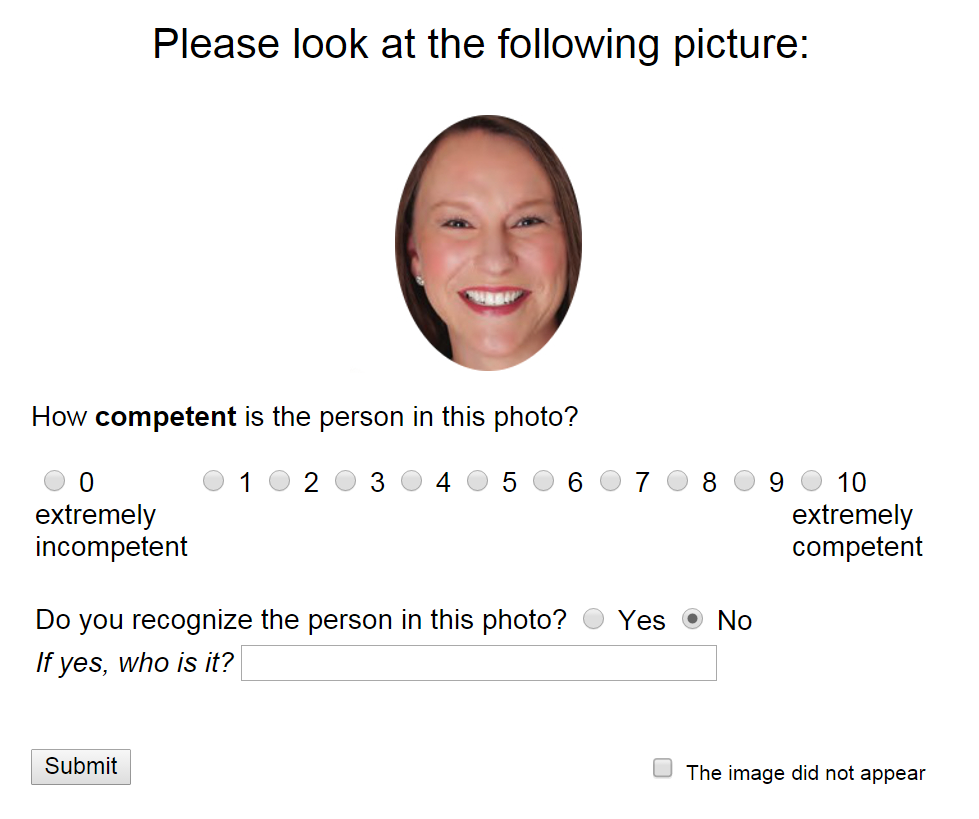
\includegraphics[width=.8\textwidth]{hit2}}
\end{center}
\caption{Example Photo Rating HIT}\label{fig:hit2}
\end{figure}

To provide a sampling of politicians' faces, I scraped photos of 533 members of 113th U.S. Congress from the website of the Government Printing Office. I then combined these photo data with 5000 randomly sampled images from the 10K U.S. Adult Faces Database \citep{BainbridgeIsolaOliva2013}, which provides a nationally representative sampling of U.S. faces, and standardized the image size and resolution across all faces.\footnote{Complete code to perform the scraping and image processing are provided along with supplemental material for this article at \url{https://github.com/leeper/mturkr-article} (\url{http://dx.doi.org/10.5281/zenodo.33595}).} To rate facial competence, I created a simple one-question HIT using HTML (see Figure \ref{fig:hit2}) that displayed one of the faces and asked for a rating of facial competence on a 0 to 10 scale.\footnote{The HIT additionally included questions to address possible problems (i.e., a subject recognizes a face or the image did not display properly).} I include the complete HTML file in supplemental materials for this article.

After uploading all 5533 images to an Amazon Simple Storage Service (S3) bucket, which is a simple cloud storage facility, to make the files publicly available\footnote{Any public file host could be used, not just S3.} and storing their filenames in a local RDS file, it was trivial to send these images to MTurk workers for categorization. To ensure reliability of the results, each face was rated by 5 workers. Workers were given 45 seconds to rate each face and were paid \$0.01 per face. The 27,665 images were rated a team of 225 U.S.-based workers over a period of 75 minutes. The entire operation cost \$412.50. Achieving this required three steps in \pkg{MTurkR}: (1) creating a QualificationRequirement to restrict the task to U.S.-based workers with 95\% approval ratings, (2) registering a HITType into which the HITs will be created, and (3) the creation of a batch of HITs using \code{BatchCreateFromURLs()}.

\begin{example}
library("MTurkR")

# Setup Qualification Requirement
## U.S.-based, 95\% approval on HITs
qual <- 
GenerateQualificationRequirement(c("Locale", "Approved"), 
                                 c("==", ">"), 
                                 c("US", 95), 
                                 preview = TRUE)

# Register HITType
desc <- "Judge the competence of a person from an image of their face.
 The HIT involves only one question: a rating of the competence of the
 person. You have 45 seconds to complete the HIT. There are several
 thousand HITs available in this batch. If you recognize the person,
 please enter their name in the space provided; your work will still be
 approved even if you recognize the face."
hittype <- 
RegisterHITType(title = "Rate the competence of a person",
                description = desc,
                reward = "0.01",
                duration = seconds(seconds = 45), 
                auto.approval.delay = seconds(days = 1),
                qual.req = qual,
                keywords = "categorization, photo, image, rating, fast, easy")

# All faces were loaded into Amazon S3
s3url <- "https://s3.amazonaws.com/mturkfaces/"
# File names were saved as a character vector locally
faces <- readRDS("faces_all.RDS")
d <- data.frame(face = paste0(s3url,faces), 
                stringsAsFactors = FALSE)

# Create 5500 HITs
bulk <- 
BulkCreateFromTemplate(template = "mturk.html",
                       frame.height = 550,
                       input = d,
                       hit.type = hittype$HITTypeId,
                       expiration = seconds(days=7),
                        # 5 assignments/face
                       assignments = 5,
                       annotation = "Face Categorization 2015-06-08")
\end{example}

\noindent Using the specified \code{annotation} value, \code{GetAssignments()} returns a large data.frame with 27670 rows and 25 columns:

\begin{example}
a <- GetAssignments(annotation = "Face Categorization 2015-06-08")
dim(a)
# [1] 27670    25
names(a)
#  [1] "AssignmentId"          "WorkerId"              "HITId"                
#  [4] "AssignmentStatus"      "AutoApprovalTime"      "AcceptTime"           
#  [7] "SubmitTime"            "ApprovalTime"          "RejectionTime"        
# [10] "RequesterFeedback"     "ApprovalRejectionTime" "SecondsOnHIT"         
# [13] "competent"             "recognized"            "name"                 
# [16] "face"                  "condition"             "browser"              
# [19] "engine"                "platform"              "language"             
# [22] "width"                 "height"                "resolution"           
# [25] "problem"
\end{example}

\noindent Most of the columns contain metadata for identifying each assignment (AssignmentId, WorkerId, HITId), metadata about the completion of the assignment (AssignmentStatus, AutoAprpovalTime, AcceptTime, SubmitTime, ApprovalTime, RejectionTime, RequesterFeedback, ApprovalRejectionTime, SecondsOnHIT), and then several columns displaying responses to the three HIT questions displayed to the workers: \code{competent}, \code{recognized}, and \code{name}. The names of these variables are given by the \code{name} attribute of the radio buttons used in the HTMLQuestion form. This HIT also additional variables that record metadata about the worker's browser, which were recorded automatically via Javascript.

As noted earlier, a limitation of the MTurk API is that it does not return information about the values of variables replaced in the templating process, so it can be difficult to identify which assignment(s) correspond to which input values. To circumvent this limitation, this HIT template was designed to use the \code{\$\{face\}} variable twice: once to actually display the image to the worker and once to record its value in a hidden field called \code{face} in the HTMLQuestion form. As a result, this variable becomes available to us in the results data.frame.

Setup in this way, it becomes trivial to analyze facial competence ratings of politicians and those from the general population sample. To perform the analysis, we simply conduct a Mann-Whitney-Wilcoxon test for a difference in competence ratings between politicians' and non-politicians' faces. (In these data, politicians' photos were identified by a simple pattern matching file name. This would have more easily been done with a hidden HTML variable when creating the batch.) So, we extract the two variables from the assignment data.frame, convert them to numeric, and perform the test:

\begin{example}
competence <- as.numeric(a$competent)
politician <- as.numeric(grepl("[[:digit:]]{2}-[[:digit:]]{3}", a$face))
wilcox.test(competence ~ politician)
# 
#         Wilcoxon rank sum test with continuity correction
# 
# data:  competence by politician
# W = 26886000, p-value < 2.2e-16
# alternative hypothesis: true location shift is not equal to 0
\end{example}

While this is a fairly trivial analytic conclusion, it demonstrates the ease with which crowdsourced human intelligence can be leveraged to preprocess a massive amount of data, translating messy sources into easily analyzed data. Because crowdsourcing is inherently massively parallel, it dramatically reduces the amount of time needed to parse a rough data source. In this case, the MTurk workers created the completed dataset in about 75 minutes. Were a single individual to attempt this task alone and it took (as a generous estimate) only 5 seconds to categorize each face, the task would be completed in 38.4 hours, or about 31-times as long as with MTurk.

\section{Conclusion}

This paper has described the MTurk platform and offered an introduction to \pkg{MTurkR} focused on preprocessing of messy data for immediate use in R. In short, \pkg{MTurkR} provides a stable, well-developed R interface to one of the largest crowdsourcing sites presently available. The package has been developed and refined for more than three years, has extensive in-package and online documentation, and is incredibly easy to use. By providing a low-level wrapper to the Amazon Mechanical Turk API, it also means that \pkg{MTurkR} could serve well as the basis for much more sophisticated R applications that leverage human intelligence as an enhancement to the computational features already available in R.

\bibliography{Leeper}

\address{Thomas J. Leeper\\
Department of Government\\
London School of Economics and Political Science\\
London, United Kingdom}\\
\email{thosjleeper@gmail.com}
